\section{Almost local metrics}
\label{sec:al-metrics}

The challenge at hand is the following: we wish to construct a notion of distance between two points in $\mathcal{I}$ by defining a metric, such that the distance between two points is the length of geodesics between the points. As we have seen, the distance induced by the $L^2$-metric vanishes on $\mathcal{I}$, so we seek to define metrics, which do not vanish. One type of such metrics is $\textit{almost local metrics}$, which, given $f \in \mathcal{I}$, are metrics of the form
\begin{align*}
G_f^\Phi (h,k) = \int_{S^1} \Phi(\text{Vol}(f), H_f, K_f) \bar{g}(h,k) \text{vol}(f^* \bar{g}),
\end{align*}
where $\Phi: \; \R^3 \rightarrow \R_{> 0}$ is smooth, $\text{Vol}(f) = \int_{S^1} \text{vol}(f^* \bar{g})$ is the total volume of $f(S^1)$, $H_f$ is the mean curvature of $f$ and $K_f$ is the Gauss curvature of $f$. Both $H_f$ and $K_f$ are local invariant properties with respect to the Riemanninan metric, defined to be the trace and the determinant of the Weingarten mapping, respectively, and so $\Phi$ is often chosen to only depend on one of the two curvatures. In the case of shapes in $\R^2$, $H_f(\theta) = \frac{\det(f_\theta, f_{\theta \theta})}{\left| f_\theta \right| ^3}$, which is just the usual formula for curvature of a plane curve.

$\Phi$ can also be seen as map from Imm$(S^1, \R^2)$ to $C^\infty (S^1, \R_{> 0})$. When viewed as such, in order for the metric to be invariant under reparametrizations, $\Phi$ must also be equivariant with respect to the action of the diffeomorphism group, Diff$(S^1)$ - i.e. $\Phi(f \circ \phi) = \Phi(f) \circ \phi$ for $\phi \in$ Diff$(S^1)$.

The total volume of $f$, $\text{Vol}(f)$, is defined via the volume form induced by the pullback metric, $f^*\bar{g}$, so this definition of almost-local metrics only applies to the manifold of embeddings from manifolds which admits a volume form. All compact, oriented manifolds do this, such as $S^1$, (Lemma $3.2$ in \cite{lee2006riemannian}), and almost local metrics are often defined for embeddings from this class of manifolds to $\R^n$. In the case of shapes in $R^2$, the volume form on $S^1$ induced by $f$ is given by vol$(f^*\bar{g}) = \left| f_\theta \right| d \theta$ (section 2.2 in \cite{michor2003riemannian}). In our case, almost local metrics therefore take on the form
\begin{align*}
G_f^\Phi (h,k) = \int_{S^1} \Phi(\text{Vol}(f), H_f, K_f) \bar{g}(h,k) \left| f_\theta \right| d \theta.
\end{align*}
Vol$(f)$ is a non-local property of $f$, and thus the metrics are not only dependent on the local properties, $K_f, H_f$, but must be $\textit{almost}$ local metrics.

\begin{remark}
Both curvatures and the volume form of a shape in $\R^2$ take on a particular nice form, but expressions can also be found for the general case where $f \in  B_e(M, \R^n)$ with $M$ a compact orientable $n-1$ dimensional manifold. This is done by using the Levi-Civita connections of the Riemannian manifolds $(\R^n,\bar{g})$ and $(M,G^\Phi)$ to construct the Weingarten mapping (see sections $3.4$ and $3.9$ of \cite{bauer2010almost}).   
\end{remark}
Note that if $\Phi$ depends only on $f$ through Vol$(f)$ then $G_f^\Phi (h,k)$ is equal to the L$^2$-metric (up to a constant). But if $\Phi$ actually depends on either curvature and the total volume, then point-separation is achieved under certain conditions imposed on $\Phi$;

\begin{theorem}\label{point_sep}
If $\Phi(\text{Vol} \, (f), H_f, K_f) = 1 + A H_f^2$ for some $A > 0$, then $G_f^\Phi$ induces a point-separating metric on $B_e(S^1, \R^2)$.
\end{theorem}

\begin{proof}
We here sketch the ideas of the proof as found in section 3 of \cite{michor2003riemannian}.

Given a path of un-parametrized shapes, $\pi(c) \, : \, [0,1] \times S^1 \rightarrow \mathcal{I}$, one can choose a path, $c$, in Imm$(S^1, \R^2)$ such that $c(0, \cdot)$ is an immersion of constant speed, $\langle c_t, c_\theta \rangle = 0$ for all $t$ and $\theta$, and $c(t , \theta)$ has constant speed. Let $c$ be such a path, and let
\begin{align*}
\Phi(f) = 1 + A H_f ^2
\end{align*}  
for some constant $A > 0$. Consider the Hilbert space $L^2(S^1, \left| c_\theta(t, \theta) \right| d\theta) = L^2(S^1, \text{vol} (c(t)^* \bar{g}))$. The Cauchy-Schwarz inequality yields
\begin{align*}
\int_{S^1} \left| c_t(t, \theta) \right| \left| c_\theta(t, \theta) \right| d \theta \leq \left(\int_{S^1} \left| c_\theta(t, \theta) \right| d \theta \right) ^{\frac{1}{2}} \left( \int_{S^1} \left| c_t(t, \theta) \right|^2 \left| c_\theta(t, \theta) \right| d \theta   \right) ^{\frac{1}{2}}.
\end{align*} 
The length of the path $c$ is then
\begin{align*}
L_{G^{\Phi}}(c) := \int_0^1  \sqrt{G^{\Phi}_{c(t)}(c_t, c_t)} dt &= \int_0^1 \left( \int (1 + AH_{c(t)}^2 ) \left| c_t(t, \theta) \right|^2 \left| c_\theta(t, \theta) \right| d\theta     \right) ^{\frac{1}{2}} dt \\
& \geq \int_0^1 \left(\int_{S^1} \left| c_\theta(t, \theta) \right| d \theta \right) ^{-\frac{1}{2}} \int_{S^1} \left| c_t(t, \theta) \right| \left| c_\theta(t, \theta) \right| d \theta dt.
\end{align*}
The mean value theorem for integrals then yields that there exists $t_0 \in [0, 1]$ such that
\begin{align*}
L_{G^{\Phi}}(c)\geq  \left(\int_{S^1} \left| c_\theta(t_0, \theta) \right| d \theta \right) ^{-\frac{1}{2}} \int_0^1 \int_{S^1} \left| c_t(t, \theta) \right| \left| c_\theta(t, \theta) \right| d \theta dt,
\end{align*}
where the first factor is the curve length of $c(t_0, \cdot)$ to the power of $-\frac{1}{2}$, and the second factor can be written as
\begin{align*}
\int_0^1 \int_{S^1} \left| c_t(t, \theta) \right| \left| c_\theta(t, \theta) \right| d \theta dt = \int_0^1 \int_{S^1} \left| \det (d c(t, \theta) \right| d \theta dt,
\end{align*}
which is the area in $\R^2$ swept out by the path $c$ (see Figure \ref{fig:area-swep}). We note that if the shape is not trivially a point in $\R^2$ (such that the length at time $t_0$ is $0$) and if the path is not trivial (such that $c(0, \cdot) = c(1, \cdot)$), then this lower bound is strictly positive. Thus any path from two distinct shapes have length greater than $0$, such that the metric induces a point-separating distance function. 
\end{proof}

\begin{figure}[h!]
  \centering
    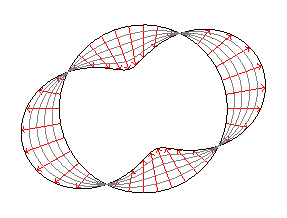
\includegraphics[scale = 1]{deform_circle.pdf}
  \caption{Illustration of the area swept out by a path $c$ in $\mathcal{I}$ with $c(0) = S^1$.}
  \label{fig:area-swep}
\end{figure}

No matter the choice of $\Phi$, an almost local metric is never point-separating on Imm$(S^1, \R^2)$ - the shape space without quotienting out reparametrizations. To see this let $f \in$ Imm$(S^1, \R^2)$ and take $\tilde{f}$ to be in the orbit of $f$ of the Diff$(S^1)$ action - i.e. $\tilde{f} = \phi \circ f$ for some $\phi \in$ Diff$(S^1)$. Since $\Phi$ is equivariant w.r.t. the action of Diff$(S^1)$, 
\begin{align*}
G_{\tilde{f}}^\Phi (h,k) = \int_{S^1} \Phi(\tilde{f}) \bar{g}(h,k) \text{vol}(f^* \bar{g}) = \int_{S^1} \Phi(f) \circ \phi \bar{g}(h,k) \text{vol}(f^* \bar{g}),
\end{align*}
the almost local metric restricted to the orbit of $f$ can be viewed as a weighted $L^2$-type metric with weights represented by $\Phi(f) \circ \phi$. As the geodesic distance function induced by weighted $L^2$ metrics vanishes (\hl{Reference or follows easily from proof?}), the almost local metric vanishes for points in Imm$(S^1, \R^2)$ which are in the same orbit of the Diff$(S^1)$-action.

In general, existence and uniqueness of geodesics w.r.t. almost local metrics are not ensured and thus the length of a path in $\mathcal{I}$ cannot be determined by constructing a geodesic and computing its length (section 5.2 in \cite{bauer2014overview}). In certain cases however, the length of a path is exactly the lower bound derived in \ref{point_sep} (see theorem 3.1 in \cite{shah2007h0type}).

\begin{example}
Define an almost local metric on $\mathcal{I}$ as above with $\Phi(f) = \ell(f)$ where $\ell(f)$ is the ordinary curve length of $f$ (which implicit is a function of the curvatures of $f$). Let $q_0, q_1 \in \mathcal{I}$ be shapes and let $c \, : \, [0,1] \rightarrow \mathcal{I}$ be a path from $q_0$ to $q_1$ such that $c(0) = q_0$ and $c(1) = q_1$. The length of the path $c$ is then the area swept out by $c$ in $\R^2$,
\begin{align*}
L_{G^\Phi}(c) = \int_{[0,1]} \int_{S^1} \left| \det dc(t, \theta) \right| d\theta dt,
\end{align*}
and the distance between $q_0$ and $q_1$ is then the infimum over all paths in $\mathcal{I}$ which start in $q_0$ and end in $q_1$:
\begin{align*}
d_{G^\Phi}(q_0, q_1) = \inf_{c\in\mathcal{C}} \int_{[0,1]} \int_{S^1} \left| \det dc(t, \theta) \right| d\theta dt,
\end{align*}
where $\mathcal{C}$ denotes all paths $c$, such that $c(0) =q_0$ and $c(1) =q_1$. \\[0.2 cm]
\end{example}
\begin{example}
If $\Phi$ is a more general function of the curve length, $\Phi = e^{A \ell (f)}$, for some constant $A > 0$, then the distance between two shapes, $q_0$ and $q_1$, is bounded by
\begin{align*}
\inf_{c\in\mathcal{C}} \sqrt{A e} \int_{[0,1]} \int_{S^1} \left| \det dc(t, \theta) \right| d\theta dt & \leq d_{G^\Phi}(q_0, q_1) \\ 
& \leq \inf_{c\in\mathcal{C}} \sqrt{A e} K \int_{[0,1]} \int_{S^1} \left| \det dc(t, \theta) \right| d\theta dt,
\end{align*}
with $K = e^{A \ell_{max}(c) / 2}$ where $\ell_{max} (c) = \max_{t \in [0,1]} \ell (c(t, \cdot))$ is the maximum length of any immersion on the path from $q_0$ to $q_1$. In particular, if $q_0 \neq q_1$, such that there exists no trivial path between the two shapes, then the distance is positive, since the area swept out in $\R^2$ by any non-trivial path is positive. 
\end{example}
Almost local metrics seem to be solutions to the challenge of finding a non-vanishing distance function on $\mathcal{I}$. After equipping $\mathcal{I}$ with such a distance function it is natural to wonder if we can in some way define the statistical concepts of section \ref{sec:mean_and_variance} on $\mathcal{I}$. We finish this exposition by a discussion on the challenges of trying to define these concepts on this infinite dimensional manifold.




